\documentclass[12pt,a4paper]{article}

% ─── Page Layout ───────────────────────────────────────────────────────────────
\usepackage[a4paper, margin=0.8in, headheight=14pt]{geometry}

% ─── Fonts (XeLaTeX) ───────────────────────────────────────────────────────────
\usepackage{fontspec}
\usepackage{unicode-math}
\setmainfont{TeX Gyre Pagella}
\setmonofont[Scale=0.88]{TeX Gyre Cursor}
\setmathfont{Latin Modern Math}

% ─── Packages ──────────────────────────────────────────────────────────────────
\usepackage{xcolor}
\usepackage{colortbl}
\usepackage{titlesec}
\usepackage{enumitem}
\usepackage{tabularx}
\usepackage{booktabs}
\usepackage{array}
\usepackage{amsmath}
\usepackage{tikz}
\usetikzlibrary{shapes.geometric, arrows.meta, positioning, calc, fit, decorations.pathreplacing}
\usepackage{tcolorbox}
\tcbuselibrary{skins, breakable}
\usepackage{hyperref}
\usepackage{fancyhdr}
\usepackage{graphicx}
\usepackage{microtype}
\hyphenpenalty=10000
\exhyphenpenalty=10000
\sloppy
\usepackage{caption}
\usepackage{setspace}
\usepackage{multirow}
\usepackage{tocloft}

% ─── Q&A helper ────────────────────────────────────────────────────────────────
\newcommand{\Q}[1]{\textbf{#1}\par\noindent\ignorespaces}

% ─── Colour Palette ────────────────────────────────────────────────────────────
\definecolor{myred}{RGB}{196,30,58}
\definecolor{mydark}{RGB}{30,30,50}
\definecolor{mygreen}{RGB}{14,120,80}
\definecolor{myteal}{RGB}{0,130,140}
\definecolor{myamber}{RGB}{180,100,0}
\definecolor{mypurple}{RGB}{100,30,160}
\definecolor{mygray}{RGB}{246,247,249}
\definecolor{mgframe}{RGB}{180,185,200}
\definecolor{watermark}{RGB}{145,150,170}
\definecolor{hdrred}{RGB}{250,232,235}
\definecolor{hdrgreen}{RGB}{220,244,233}
\definecolor{hdrteal}{RGB}{220,242,244}
\definecolor{hdramber}{RGB}{253,242,215}
\definecolor{hdrpurple}{RGB}{238,228,255}
\definecolor{hdrgray}{RGB}{238,240,245}
\definecolor{rowalt}{RGB}{250,251,253}

% ─── Section Formatting ────────────────────────────────────────────────────────
\titleformat{\section}
  {\large\bfseries\color{myred}}{\thesection.}{0.5em}{}
  [\vspace{1pt}{\color{myred}\rule{\linewidth}{0.8pt}}]
\titleformat{\subsection}
  {\normalsize\bfseries\color{myteal}}{\thesubsection}{0.5em}{}
\titlespacing*{\section}{0pt}{18pt}{7pt}
\titlespacing*{\subsection}{0pt}{11pt}{4pt}

% ─── Paragraph ─────────────────────────────────────────────────────────────────
\setlength{\parindent}{0pt}
\setlength{\parskip}{4pt}

% ─── TOC Styling ───────────────────────────────────────────────────────────────
\renewcommand{\cfttoctitlefont}{\large\bfseries\color{myred}}
\renewcommand{\cftaftertoctitle}{\par\noindent{\color{myred}\rule{\linewidth}{0.8pt}}}
\setlength{\cftbeforetoctitleskip}{0pt}
\setlength{\cftaftertoctitleskip}{6pt}
\renewcommand{\cftsecfont}{\normalsize\bfseries\color{mydark}}
\renewcommand{\cftsecpagefont}{\normalsize\bfseries\color{mydark}}
\renewcommand{\cftsecleader}{\cftdotfill{\cftdotsep}}
\setlength{\cftbeforesecskip}{7pt}
\renewcommand{\cftsubsecfont}{\small\color{mydark}}
\renewcommand{\cftsubsecpagefont}{\small\color{mydark}}
\setlength{\cftbeforesubsecskip}{3pt}
\setlength{\cftsubsecindent}{1.4em}

% ─── Table helpers ─────────────────────────────────────────────────────────────
\renewcommand{\arraystretch}{1.45}
\setlength{\tabcolsep}{6pt}
\arrayrulecolor{mydark}
\newcolumntype{B}[1]{>{\small\bfseries\raggedright\arraybackslash}m{#1}}
\newcolumntype{Y}{>{\small\raggedright\arraybackslash}X}
\renewcommand{\tabularxcolumn}[1]{m{#1}}

% ─── Header / Footer ───────────────────────────────────────────────────────────
\pagestyle{fancy}
\fancyhf{}
\fancyhead[L]{\small\color{myred}\textbf{PE-EC701A}\;\color{mydark}--- Microwave Theory and Technique}
\fancyhead[R]{\small\color{myteal}\textbf{Module 1 Notes}}
\fancyfoot[C]{\small\color{mydark}\thepage}
\fancyfoot[R]{\small\color{watermark}\textit{\copyright\ Biraj}}
\renewcommand{\headrulewidth}{0.5pt}
\renewcommand{\footrulewidth}{0.3pt}

% ─── Hyperref ──────────────────────────────────────────────────────────────────
\hypersetup{
  colorlinks=true, linkcolor=myteal, urlcolor=myteal,
  pdfauthor={Biraj Sarkar},
  pdftitle={PE-EC701A --- Module 1 Notes}
}

% ─── tcolorbox styles ──────────────────────────────────────────────────────────
\tcbset{
  tikzbox/.style={
    colback=mygray, colframe=mgframe, boxrule=0.6pt, arc=4pt,
    left=8pt, right=8pt, top=6pt, bottom=6pt,
    colbacktitle=mgframe, coltitle=mydark,
    fonttitle=\small\bfseries
  },
  defbox/.style={
    colback=hdrgreen, colframe=mygreen, boxrule=0.8pt, arc=4pt,
    left=9pt, right=9pt, top=6pt, bottom=6pt,
    colbacktitle=mygreen, coltitle=white,
    fonttitle=\small\bfseries
  },
  formulabox/.style={
    colback=hdrteal, colframe=myteal, boxrule=0.8pt, arc=4pt,
    left=9pt, right=9pt, top=7pt, bottom=7pt,
    colbacktitle=myteal, coltitle=white,
    fonttitle=\small\bfseries
  },
  examplebox/.style={
    colback=hdramber, colframe=myamber, boxrule=0.8pt, arc=4pt,
    left=9pt, right=9pt, top=6pt, bottom=6pt,
    colbacktitle=myamber, coltitle=white,
    fonttitle=\small\bfseries
  },
  masonbox/.style={
    colback=hdrpurple, colframe=mypurple, boxrule=0.8pt, arc=4pt,
    left=9pt, right=9pt, top=6pt, bottom=6pt,
    colbacktitle=mypurple, coltitle=white,
    fonttitle=\small\bfseries
  },
  exambox/.style={
    colback=hdrpurple, colframe=mypurple, boxrule=1pt, arc=5pt,
    left=10pt, right=10pt, top=8pt, bottom=8pt,
    colbacktitle=mypurple, coltitle=white,
    fonttitle=\bfseries,
    breakable, title after break={\textbf{Frequently Asked / Viva Questions (contd.)}}}
}
% Make all boxes breakable across pages
\tcbset{breakable}

% ─── TikZ styles ───────────────────────────────────────────────────────────────
\tikzset{
  block/.style={rectangle, draw=myteal, fill=hdrteal,
    text width=2.4cm, align=center, minimum height=0.95cm,
    font=\small, rounded corners=3pt, line width=0.7pt},
  redblock/.style={rectangle, draw=myred, fill=hdrred,
    text width=2.4cm, align=center, minimum height=0.95cm,
    font=\small, rounded corners=3pt, line width=0.7pt},
  netnode/.style={rectangle, draw=myteal, fill=hdrteal,
    text width=1.5cm, align=center, minimum height=0.8cm,
    font=\small, rounded corners=3pt, line width=0.7pt},
  sumjunc/.style={circle, draw=myamber, fill=hdramber,
    minimum size=0.62cm, font=\small, line width=0.8pt},
  snode/.style={circle, draw=mypurple, fill=hdrpurple,
    minimum size=0.55cm, font=\footnotesize, line width=0.7pt},
  arrow/.style={-Stealth, thick, color=mydark},
  redarrow/.style={-Stealth, thick, color=myred},
  line/.style={thick, color=mydark}
}

% ═══════════════════════════════════════════════════════════════════════════════
\begin{document}
% ═══════════════════════════════════════════════════════════════════════════════

\begin{center}
  {\LARGE\bfseries\color{myred} PE-EC701A --- Microwave Theory and Technique}\\[5pt]
  {\normalsize\color{mydark} Semester VII \quad$\bullet$\quad 3L:0T:0P \quad$\bullet$\quad 3 Credits}\\[3pt]
  {\normalsize\color{myteal}\textbf{Module 1 Exam Notes: Introduction to Microwaves}}\\[3pt]
  {\small\color{mydark} CGEC \;$|$\; B.Tech ECE (2023--27) \;$|$\; \textit{Biraj Sarkar}}
\end{center}
\vspace{2pt}
\noindent{\color{myred}\rule{\linewidth}{1.5pt}}
\vspace{2pt}

\hypersetup{linkcolor=mydark}
\tableofcontents
\hypersetup{linkcolor=myteal}
\newpage

% ===============================================================================
\section{Introduction to Microwaves}
% ===============================================================================

Microwaves represent a key segment of the electromagnetic spectrum that lies between radio frequencies and infrared radiation. They are characterized by short wavelengths, which gives rise to their name.

\begin{tcolorbox}[defbox]
\textbf{Microwaves:} Electromagnetic waves with frequencies ranging from \textbf{300 MHz (0.3 GHz) to 300 GHz}, which corresponds to free-space wavelengths ranging from \textbf{1 m to 1 mm} respectively. They propagate in line-of-sight paths and are governed by Maxwell's electromagnetic equations.
\end{tcolorbox}

\subsection{History and Evolution of Microwaves}
The physical foundation of microwaves dates back to the theoretical and experimental milestones of the 19th and 20th centuries:
\begin{itemize}[leftmargin=*, itemsep=3pt]
  \item \textbf{James Clerk Maxwell (1864):} Formulated the electromagnetic theory predicting the existence of electromagnetic waves.
  \item \textbf{Heinrich Hertz (1888):} Experimentally proved Maxwell's equations by generating and detecting radio waves at UHF/microwave frequencies using spark-gap transmitters.
  \item \textbf{Jagadish Chandra Bose (1895):} Generated millimeter-wave signals up to 60 GHz and demonstrated remote signaling and polarization effects using horn antennas and semiconductor detectors.
  \item \textbf{World War II (1939--1945):} Accelerated microwave research due to the operational necessity of Radar. The invention of the Cavity Magnetron by Randall and Boot enabled high-power radar transmitters.
  \item \textbf{Post-War Era:} Shifted focus toward civilian telecommunications, satellite links, cellular networks, and domestic heating (microwave oven).
\end{itemize}

\subsection{Electromagnetic Spectrum Representation}
The position of the microwave band within the wider electromagnetic spectrum is illustrated below:

\begin{tcolorbox}[tikzbox, title={Electromagnetic Spectrum Highlighting Microwave Band}]
\centering
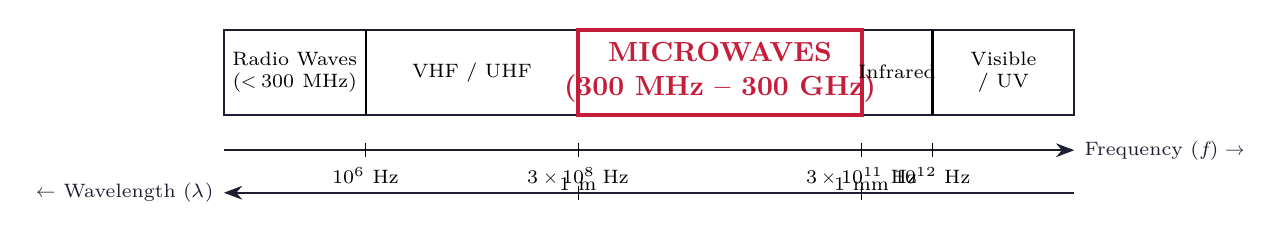
\begin{tikzpicture}[scale=0.9, every node/.style={font=\scriptsize}]
  % Draw spectrum bar
  \draw[thick, color=mydark] (0,0) rectangle (12,1.2);
  
  % Dividers and Labels
  \draw[thick] (2,0) -- (2,1.2);
  \draw[thick] (5,0) -- (5,1.2);
  \draw[thick, color=myred, line width=1.5pt] (5,0) rectangle (9,1.2);
  \draw[thick] (10,0) -- (10,1.2);
  
  \node[align=center] at (1,0.6) {Radio Waves\\($<300$ MHz)};
  \node[align=center, font=\bfseries\color{myred}] at (7,0.6) {MICROWAVES\\(300 MHz -- 300 GHz)};
  \node at (3.5,0.6) {VHF / UHF};
  \node at (9.5,0.6) {Infrared};
  \node[align=center] at (11,0.6) {Visible\\/ UV};
  
  % Frequency and Wavelength axis markers below
  \draw[arrow] (0,-0.5) -- (12,-0.5) node[right] {Frequency ($f$) $\to$};
  \draw[arrow] (12,-1.1) -- (0,-1.1) node[left] {$\gets$ Wavelength ($\lambda$)};
  
  % Ticks for frequency
  \draw (2,-0.4) -- (2,-0.6) node[below] {$10^6$ Hz};
  \draw (5,-0.4) -- (5,-0.6) node[below] {$3 \times 10^8$ Hz};
  \draw (9,-0.4) -- (9,-0.6) node[below] {$3 \times 10^{11}$ Hz};
  \draw (10,-0.4) -- (10,-0.6) node[below] {$10^{12}$ Hz};
  
  % Ticks for wavelength
  \draw (5,-1.0) -- (5,-1.2) node[above] {$1$ m};
  \draw (9,-1.0) -- (9,-1.2) node[above] {$1$ mm};
\end{tikzpicture}
\tcbset{colbacktitle=myteal, coltitle=white}
\end{tcolorbox}

% ===============================================================================
\section{Microwave Frequency Bands}
% ===============================================================================

To avoid spectral confusion, the microwave spectrum is subdivided into distinct bands. The two primary naming standards are the \textbf{IEEE Standard} (used in radar and communications) and the \textbf{Military/NATO Standard}.

\subsection{IEEE Microwave Frequency Band Classification}
The table below details the frequency and wavelength ranges defined by the IEEE:

\par\noindent
{\renewcommand{\arraystretch}{1.55}%
\begin{tabularx}{\linewidth}{|B{3.2cm}|Y|Y|Y|}\hline
\textbf{Band Designation} & \textbf{Frequency Range} & \textbf{Wavelength Range} & \textbf{Typical Applications} \\[4pt]
\hline
\textbf{L Band} & $1.0 - 2.0$ GHz & $30.0 - 15.0$ cm & GPS, Mobile phones (GSM), Satellite navigation \\[4pt]
\hline
\textbf{S Band} & $2.0 - 4.0$ GHz & $15.0 - 7.5$ cm & Wi-Fi (2.4 GHz), Microwave ovens, Weather radars \\[4pt]
\hline
\textbf{C Band} & $4.0 - 8.0$ GHz & $7.5 - 3.75$ cm & Satellite TV transponders, Wi-Fi (5.8 GHz) \\
\hline
\textbf{X Band} & $8.0 - 12.0$ GHz & $3.75 - 2.50$ cm & Military radar, Marine navigation, Speed detectors \\[4pt]
\hline
\textbf{Ku Band} & $12.0 - 18.0$ GHz & $2.50 - 1.67$ cm & Direct-to-Home (DTH) TV, Satellite networks \\[4pt]
\hline
\textbf{K Band} & $18.0 - 27.0$ GHz & $1.67 - 1.11$ cm & Radar altimeters, Water vapour absorption line (22 GHz) \\[4pt]
\hline
\textbf{Ka Band} & $27.0 - 40.0$ GHz & $1.11 - 0.75$ cm & High-speed satellite broadband, Close-range radar \\[4pt]
\hline
\textbf{V Band} & $40.0 - 75.0$ GHz & $7.5 - 4.0$ mm & Short-range military comms, 60 GHz Wi-Fi (IEEE 802.11ad) \\[4pt]
\hline
\textbf{W Band} & $75.0 - 110$ GHz & $4.0 - 2.7$ mm & Automotive radars, Millimeter-wave imaging \\
\hline
\end{tabularx}
}

% ===============================================================================
\section{Key Advantages and Properties of Microwaves}
% ===============================================================================

Microwaves possess specific properties that differentiate them from lower-frequency radio waves:

\begin{enumerate}[label=\textbf{\arabic*.}, leftmargin=*, itemsep=4pt]
  \item \textbf{High Information Carrying Capacity (Large Bandwidth):} The available bandwidth in the microwave region is several orders of magnitude larger than the entire HF and VHF radio spectrum combined.
    \begin{equation}
      \text{Bandwidth } \Delta f = f_2 - f_1
    \end{equation}
    Since frequency is high, a small fractional bandwidth yields enormous absolute bandwidth, enabling high-rate data transmission.
  \item \textbf{Line-of-Sight (LoS) Propagation:} Microwaves travel in straight lines and are not reflected by the ionosphere. This ensures clean, interference-free point-to-point communication but requires repeater towers due to earth's curvature.
  \item \textbf{Directive Antenna Gain:} The gain of an antenna is inversely proportional to the square of the wavelength:
    \begin{equation}
      G = \frac{4\pi A_e}{\lambda^2}
    \end{equation}
    Because $\lambda$ is small, very high antenna gain and narrow beamwidths can be achieved with physically small structures (e.g., dish antennas).
  \item \textbf{Lower Power Requirements:} Highly directive antennas concentrate energy into a narrow beam, requiring significantly lower transmitter power to span long links compared to omnidirectional HF systems.
  \item \textbf{Ionospheric Transparency:} Frequencies above 100 MHz pass directly through the ionosphere without being reflected or bent, making space, satellite, and deep-space communications possible.
\end{enumerate}

% ===============================================================================
\section{Applications of Microwaves}
% ===============================================================================

\subsection{Civil and Military Applications}
The primary applications of microwaves are split across the civilian and defense sectors:

\textbf{Civilian Applications:}
\begin{itemize}[leftmargin=*, itemsep=2pt]
  \item \textbf{Telecommunications:} Cellular networks (LTE, 5G), Wi-Fi router bands, and satellite voice/data networks.
  \item \textbf{Satellite Broadcasting:} Direct-to-Home (DTH) TV services (operating in the Ku band) and satellite radio.
  \item \textbf{Meteorology:} Weather radar systems operating in the S and C bands to map precipitation and storm tracks.
  \item \textbf{Domestic Heating:} Microwave ovens operate at 2.45 GHz, utilizing dielectric heating of water molecules in food.
\end{itemize}

\textbf{Military Applications:}
\begin{itemize}[leftmargin=*, itemsep=2pt]
  \item \textbf{Radar Detection and Tracking:} Fire-control radars, air traffic monitoring, and target tracking (operating in X and Ku bands).
  \item \textbf{Electronic Warfare (EW):} Jamming enemy communications, electronic countermeasures (ECM), and radar signature reduction (stealth).
  \item \textbf{Missile Guidance:} Semi-active and active radar seekers located in the nose cones of missiles.
\end{itemize}

\subsection{Medical Applications}
Microwaves interact with biological tissues in ways that enable both diagnostics and therapy:
\begin{itemize}[leftmargin=*, itemsep=3pt]
  \item \textbf{Microwave Hyperthermia:} Delivering controlled heat to tumors. Cancer cells are more heat-sensitive than healthy tissue, and raising their temperature to $42^\circ\text{C}$--$45^\circ\text{C}$ helps destroy them.
  \item \textbf{Microwave Ablation (MWA):} Using localized needle-like microwave antennas inserted into tumors to cook and destroy cancer cells directly.
  \item \textbf{Microwave Imaging:} Utilizing dielectric contrast between healthy and malignant breast tissues to detect tumors without ionizing radiation.
\end{itemize}

% ===============================================================================
\section{EMI/EMC Concepts at Microwave Frequencies}
% ===============================================================================

As operating frequencies increase, electromagnetic interactions become critical, necessitating strict EMI/EMC compliance.

\begin{tcolorbox}[defbox]
\textbf{EMI (Electromagnetic Interference):} Any electromagnetic disturbance or emission that degrades, disrupts, or limits the effective performance of electrical equipment.

\textbf{EMC (Electromagnetic Compatibility):} The ability of an electrical system or device to function satisfactorily in its electromagnetic environment without introducing intolerable electromagnetic disturbances to anything in that environment.
\end{tcolorbox}

\subsection{The EMI Coupling Path}
For electromagnetic interference to occur, three elements must be present:

\begin{tcolorbox}[tikzbox, title={Elements of Electromagnetic Interference}]
\centering
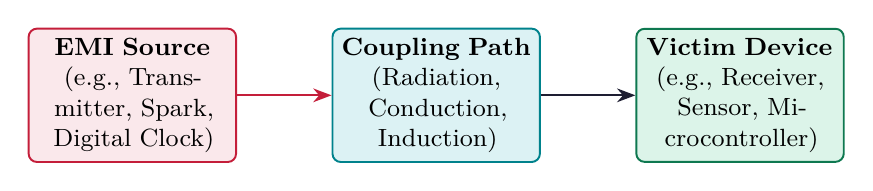
\begin{tikzpicture}[node distance=0.6cm and 1.2cm]
  \node[redblock] (src) {\textbf{EMI Source}\\(e.g., Transmitter, Spark, Digital Clock)};
  \node[block, right=1.2cm of src] (path) {\textbf{Coupling Path}\\(Radiation, Conduction, Induction)};
  \node[block, draw=mygreen, fill=hdrgreen, right=1.2cm of path] (vic) {\textbf{Victim Device}\\(e.g., Receiver, Sensor, Microcontroller)};
  
  \draw[arrow, color=myred] (src) -- (path);
  \draw[arrow] (path) -- (vic);
\end{tikzpicture}
\end{tcolorbox}

\subsection{EMI Mitigation Techniques}
\begin{itemize}[leftmargin=*, itemsep=2pt]
  \item \textbf{Shielding:} Enclosing sensitive circuits in metallic containers (Faraday cages) to reflect and absorb radiated fields.
  \item \textbf{Grounding:} Ensuring low-impedance ground return paths to prevent common-mode voltage differences.
  \item \textbf{Filtering:} Installing low-pass filters on power and signal lines to suppress high-frequency noise.
\end{itemize}

% ===============================================================================
% MANDATORY QUICK REVISION PAGE
% ===============================================================================
\newpage
\begin{center}
  {\large\bfseries\color{myred} Quick Revision --- Module I}\\[3pt]
  {\small\color{mydark} Introduction to Microwaves $|$ PE-EC701A}
\end{center}
\noindent{\color{myred}\rule{\linewidth}{1.2pt}}
\vspace{4pt}

\begin{tcolorbox}[formulabox, title={\textbf{Key Formulas at a Glance}}]
\renewcommand{\arraystretch}{1.3}
\begin{tabularx}{\linewidth}{B{4.5cm} X}Wave Velocity Relation  & $c = f \lambda \approx 3 \times 10^8 \text{ m/s}$ (in free space) \\[4pt]
Antenna Directivity/Gain & $G = \frac{4\pi A_e}{\lambda^2}$ \quad ($A_e$ = effective aperture area) \\[4pt]
Bandwidth               & $\Delta f = f_2 - f_1$ \\[4pt]
Decibel Power Ratio     & $P_{\text{dB}} = 10 \log_{10}\left(\frac{P_{\text{out}}}{P_{\text{in}}}\right)$
\end{tabularx}
\end{tcolorbox}

\begin{tcolorbox}[defbox, title={\textbf{One-Line Definitions}}]
\begin{itemize}[leftmargin=*, itemsep=2.5pt, topsep=0pt]
  \item \textbf{Microwave:} Electromagnetic waves operating between 300 MHz and 300 GHz.
  \item \textbf{Dominant Mode:} The waveguide transmission mode that exhibits the lowest cutoff frequency.
  \item \textbf{Line-of-Sight:} Straight-line propagation between antennas with no ionospheric reflection.
  \item \textbf{EMI:} Disturbance of electronic systems caused by unintended electromagnetic fields.
  \item \textbf{EMC:} The capacity of a device to operate without radiating or absorbing excessive EMI.
  \item \textbf{Microwave Hyperthermia:} Thermal therapy utilizing microwaves to selectively heat and destroy tumor cells.
  \item \textbf{Faraday Cage:} A conductive enclosure used to block external radiated electromagnetic fields.
\end{itemize}
\end{tcolorbox}

\begin{tcolorbox}[exambox, title={\textbf{Frequently Asked / Viva Questions}}]
\begin{enumerate}[topsep=0pt, label=\textbf{Q\arabic*.}, itemsep=5pt]
  \item \Q{State the frequency and wavelength ranges of microwaves.}
    Frequencies range from 300 MHz to 300 GHz, corresponding to free-space wavelengths of 1 m to 1 mm respectively.
  \item \Q{Why are microwaves not reflected by the ionosphere?}
    Because of their high frequencies ($>100$ MHz). The ionospheric plasma frequency is lower, allowing microwaves to pass directly through without reflection.
  \item \Q{What are the typical frequency ranges for the L, S, C, and X bands?}
    L band: $1 - 2$ GHz; S band: $2 - 4$ GHz; C band: $4 - 8$ GHz; X band: $8 - 12$ GHz.
  \item \Q{Why are microwave antennas physically small for a given high gain?}
    Gain is inversely proportional to $\lambda^2$ ($G = 4\pi A_e/\lambda^2$). Since $\lambda$ is small, a small aperture $A_e$ is sufficient to achieve high gain.
  \item \Q{List three major advantages of using microwaves for communication.}
    Large operational bandwidth (high information capacity), high antenna directivity, and immunity to ionospheric disturbances.
  \item \Q{What is the operating frequency of a domestic microwave oven and why?}
    2.45 GHz. This frequency matches the rotational excitation energy of water molecules, ensuring efficient dielectric heating of food.
  \item \Q{Explain the difference between EMI and EMC.}
    EMI is the interference signal itself that disrupts electronic operation. EMC is the design property of a system to resist EMI and avoid emitting it.
  \item \Q{State the medical applications of microwaves.}
    Microwave hyperthermia for cancer therapy, microwave ablation to destroy tissue, and non-invasive microwave breast imaging.
  \item \Q{Why is point-to-point microwave communication limited by distance?}
    Because microwaves propagate in straight lines (LoS). Due to the earth's curvature, repeater stations are required approximately every 50 km.
  \item \Q{What is the significance of the X-band in military applications?}
    X-band ($8 - 12$ GHz) offers a good compromise between atmospheric attenuation and spatial resolution, making it ideal for tracking and fire-control radars.
  \item \Q{How does high operating frequency affect digital circuits regarding EMI?}
    As frequency increases, trace lines on PCBs act as antennas, leading to crosstalk, radiation emission, and high susceptibility to noise.
  \item \Q{What is shielding effectiveness (SE)?}
    It is the ratio of the electromagnetic field strength before shielding to the field strength after shielding, measured in decibels (dB).
\end{enumerate}
\end{tcolorbox}

\begin{tcolorbox}[tikzbox, title={Comparison of Civil and Military Microwave Applications}]
\renewcommand{\arraystretch}{1.4}
\par\noindent
{\renewcommand{\arraystretch}{1.55}%
\begin{tabularx}{\linewidth}{|B{3.0cm}|Y|Y|}\hline
\textbf{Parameter} & \textbf{\color{myteal}Civil Applications} & \textbf{\color{myred}Military Applications} \\[4pt]
\hline
\textbf{Primary Goal} & High-capacity data transfer, media broadcast, and domestic heating. & Surveillance, threat tracking, weapons guidance, and communications jamming. \\[4pt]
\hline
\textbf{Typical Bands} & L, S, C, Ku bands (high-speed data, DTH satellite). & X, Ku, Ka, W bands (fine-resolution radar, stealth systems). \\[4pt]
\hline
\textbf{Design Priority} & Cost efficiency, standardized channels, and regulatory compliance. & High reliability, anti-jamming capabilities, and high-power output. \\[4pt]
\hline
\textbf{Standard Devices} & Solid-state transceivers, standard Wi-Fi routers. & High-power magnetrons, traveling-wave tubes (TWT), and phased-array systems. \\[4pt]
\hline
\end{tabularx}
}
\end{tcolorbox}

\end{document}
